\chapter{User study}
\label{sec:user_study_chapter}
%
% USER STUDY CHAPTER
%

From August 21th to September 12th 2017, I conducted a user study that aimed at gathering data to compare with the results of processing 3D objects according to \textit{mesh saliency} \cite{lee2005mesh}. However, due to the fact that the projection installation at the V2C was not available for me at all times, I could not use every day in that timespan. The installation was assigned to me for a total seven days. I was able to collect a reasonable amount of data from a sufficiently sized group of participants. This chapter will go over details of how I organised and conducted the user study.

As briefly described before in section \ref{sec:conduct_user_study_with_the_selection_application}, I asked participants to use my selection application and the hardware available at the V2C to select regions of 3D objects they found \textit{interesting}. In general, participants got familiar with the devices and interaction mechanics quickly and were able to make selections according to their perception of what was of importance.
% @TODO: Kurzen Spoiler einbauen, wie es sich mit den Unterschieden verhalten hat (das Ziel der ganzen verf*ckten Arbeit halt)

	\section{Hardware used}
	\label{sec:hardware_used}
%
% HARDWARE USED
%

The five-sided projection installation at the V2C is equipped with several devices which can be tracked inside of it. Users taking part in the user study were asked to put on a pair of lightweight stereoscopic glasses, shown in figure \ref{fig:glasses}. Note the three white, spherical parts on each side of the glasses. These are used for tracking their position, orientation, tilt and yaw within the projection installation. According to these parameters, two images are projected onto the walls of the installation from behind, each for one eye. The glasses are in synchronisation with the projectors and actively switch between left and right 120 times per second, only showing one of the projected images at a time. This way, an immersive 3D effect for one user wearing the glasses within the installation is created.  

For interaction, a handheld device called \textit{wand} see figure \ref{fig:wand}, is used within the projection installation. It allows for navigation within the scene via a little joystick as well as interaction with four buttons. The joystick moves the scene in the opposite way the user pushes it. This has been described as counter-intuitive by some users.

As described in \ref{sec:selection_process}, two of those buttons are enough for the selection application's needs. The button on top of the \textit{wand}, on the left side of the joystick is used for making selections on the currently loaded 3D object, the button  right to it can be used to clear already marked selections. Figure \ref{fig:wand} shows the device. Again, note the white, spherical parts used for tracking position, orientation, tild and yaw of the device attached to it.

\begin{figure}[htb]
  \centering
  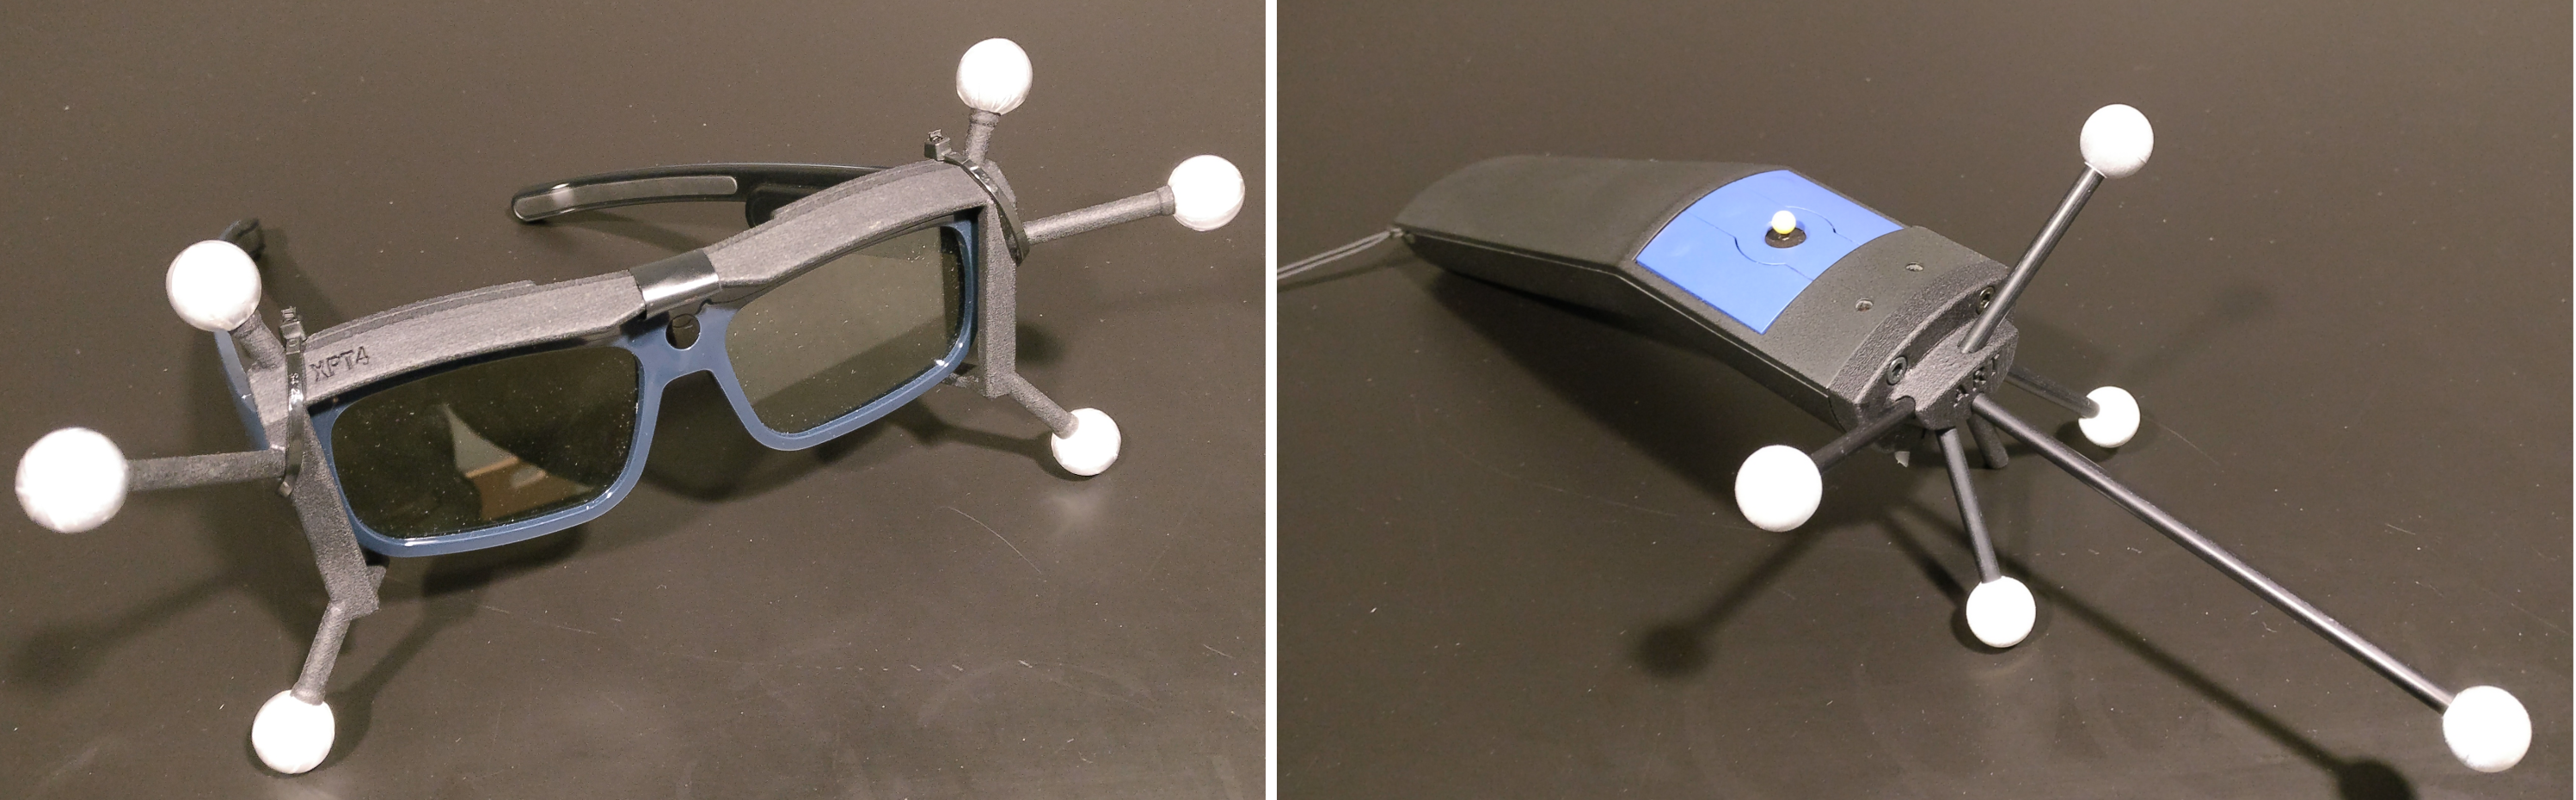
\includegraphics[width=.95\textwidth]{concept_hardware.png}\\ % PNG-File
  \caption{The hardware components available at the V2C. Left: A pair of active, stereoscopic shutter glasses. Right: The main input device, referred to as \textit{wand}}
  \label{fig:selection_cave}
\end{figure}

\begin{figure}[htb]
  \centering
  \includegraphics[width=.8\textwidth]{selection_cave.png}\\ % PNG-File
  \caption{The selection process using the available hardware at the V2C}\label{fig:selection_cave}
\end{figure}

Figure \ref{fig:selection_cave} depicts what the selection process inside the projection installation at the V2C is like form a user perspective. Users utilise the \textit{wand} for navigation as well as selecting and deselecting parts of the presented objects they deem \textit{interesting}. The stereoscopic glasses provide a spatially convincing, three-dimensional immersion of the object. In the figure, the object is a simple cube with two iterative subdivisions. Its vertices are shaded grey, the edges connecting them are shaded black. The diamond-shaped object indicating the position of the \textit{wand} within the 3D scene is shaded bright green. The blue circle around it represents the spherical query radius for selection and deselection operations. Vertices within that lie within that circle are shaded orange.

% @TODO: 3 Fotos von einem Teilnehmer vom Selection Process machen (nichts selektiert; etwas selektiert; Selektion bearbeitet)

% @TODO: (Reminder, siehe 03-concept, hier darauf verweisen oder umgekehrt)
% @TODO: Bild rausrendern (user mit Wand in der Hand, geladenem Object + wand_pos), schneiden und uploaden

	\section{Models used}
	\label{sec:models_used}
%
% MODELS USED
%

Regarding objects used for the study, I aimed at offering as much variety of types of objects among as few objects as possible. The motivation for this was to achieve results that are genereally applicable for any type of geometric data, at least to an basic extent. Also, to avoid the users losing motivation due to repeating tasks during the study, keeping the number of objects to a minimum was a constraint to be considered. I decided to use three objects described table in \ref{tab:userstudy_objects} and depicted in figure \ref{fig:all_objects}. Note that the models are from third-party vendors. I made sure they are all free to use for educational purposes and weblinks to where they have been published originally are provided in the bibliography.

Figure \ref{fig:all_objects} shows the objects used in the user study. From left to right, the 3D scanned bunny, the modelled cow and the low-poly, modelled aircraft are shown. Consider the grid to get a sense of their proportions. I did not scale them according to their real world sizes and instead made them take up approximately equal space in the virtual scene. This was done with the intention to provide a similar level of visual detail, independent of the actual geometric level of detail, for each object. Furthermore, I wanted to prevent the size of the objects from having any sort of influence on how users perceived them.

\begin{table}[]
\centering
	\begin{tabular}{l|l|l|l|l}
		object	& created through	& source	& vertex count	& class of objects	\\ \hline
		cow	& 3D modelling		& \cite{cow}	& 69,648	& purely natural	\\
		P51 Mustang	&	3D modelling	& \cite{P51}	& 51,708	& purely mechanical	\\
		bunny sculpture	&	3D scan	& \cite{bun}	& 68,754	& natural, man-made	
	\end{tabular}
	\caption{3D objects used in the study}
	\label{tab:userstudy_objects}
\end{table}
% table 3.1

\begin{figure}[htb]
  \centering
  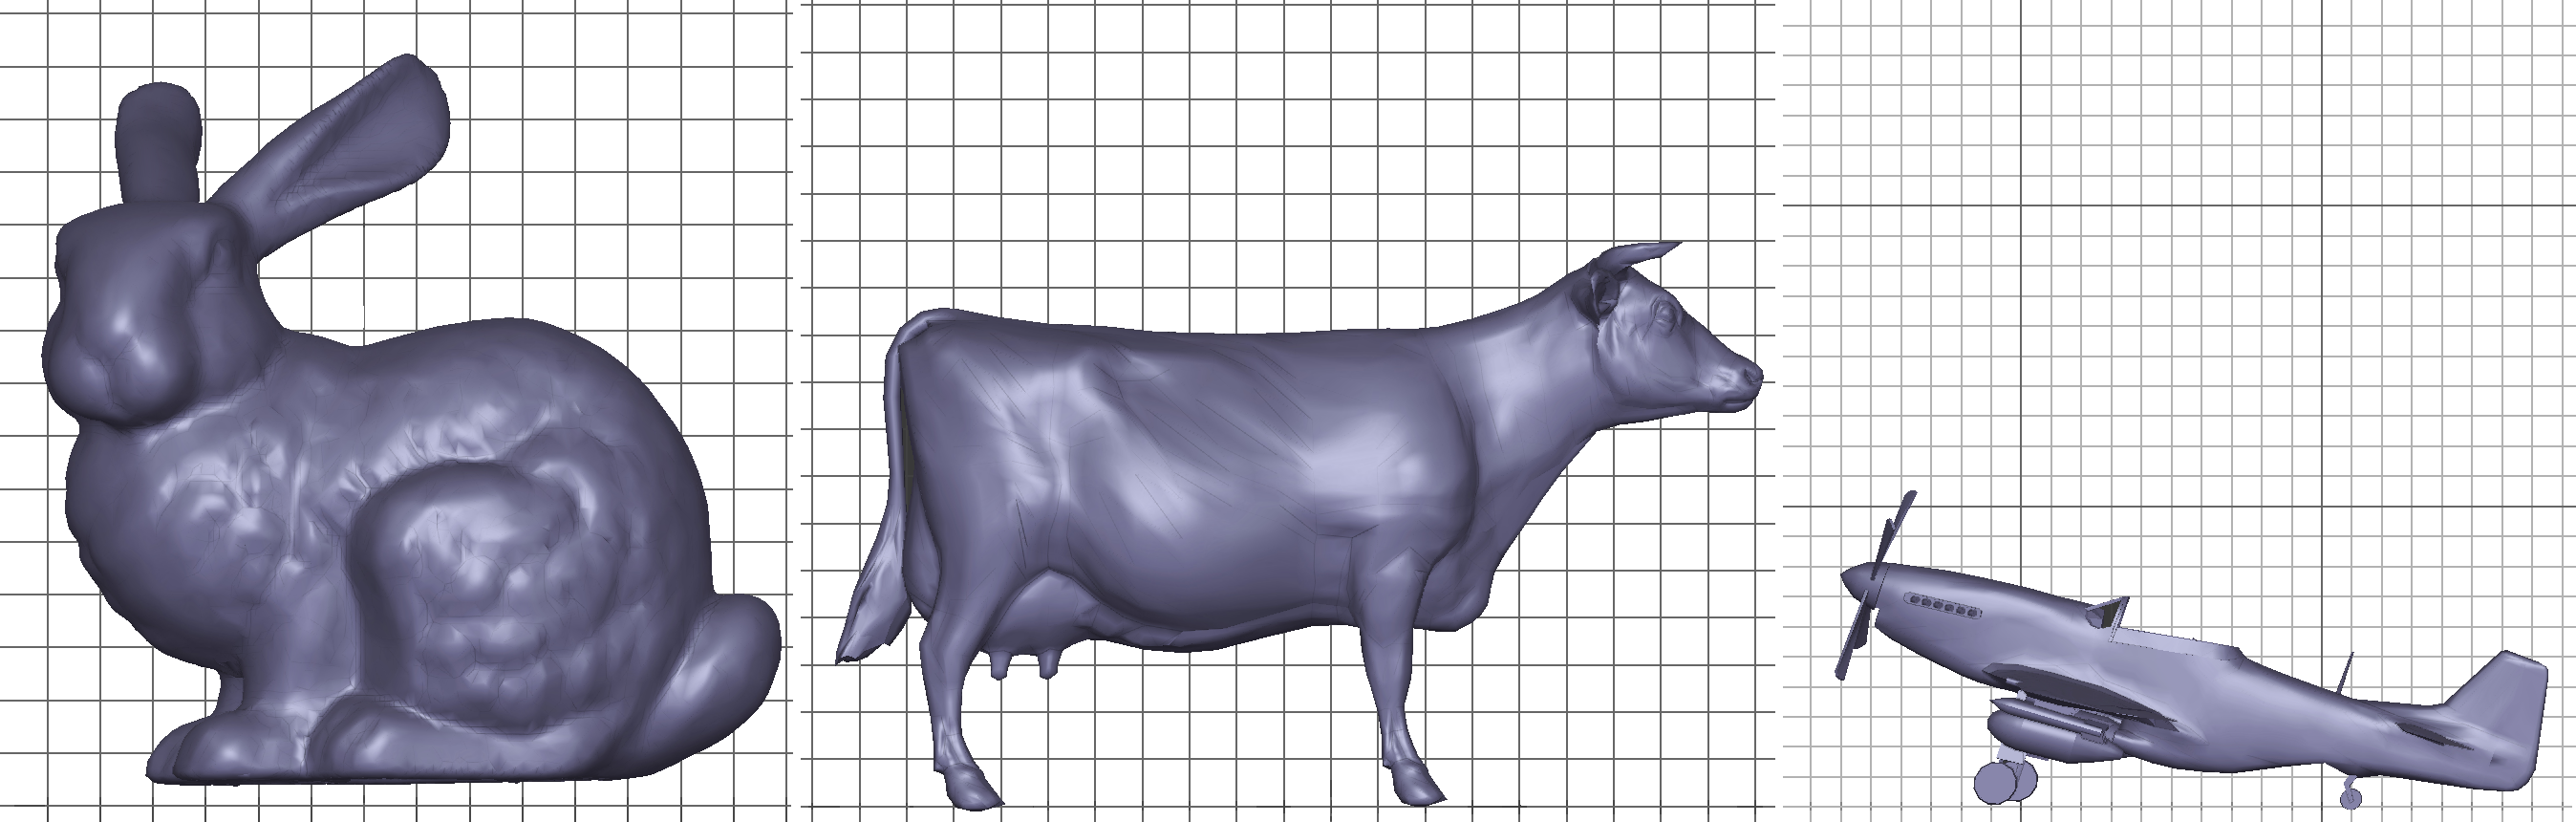
\includegraphics[width=1.0\textwidth]{userstudy_all_objects.png}\\ % PNG-File
  \caption{The 3D objects used for the user study}\label{fig:all_objects}
\end{figure}

	\section{Tasks given}
	\label{sec:tasks_given}
%
% TASKS GIVEN
%

Users were asked to use the hard- and software available to select regions and parts of the objects they deemed \textit{interesting} since \textit{mesh saliency} claims to be able to reliably predict such parts \cite{lee2005mesh}. I told the users that this would be the task at hand only after they stated they felt ready to interact with the scene presented in the projection installation. They were given as much time as they wanted to get somewhat accustomed to navigating and the selection process it but in general, nobody took longer than a few minutes.

I then explained the course of the user study, going over the following instructions:
\begin{itemize}
	\item The task is to select parts and regions of the objects users consider \textit{important}.
	\item Some suggestions as to what could be considered \textit{important}:
		\begin{itemize}
			\item \textit{what do you consider visually interesting or important?}
			\item \textit{what do you assume are natural focus points of attention?}
			\item \textit{what parts do you consider vital for identifying the object?}
		\end{itemize}
	\item However these are just ideas, in general users were encouraged to select whatever they, personally, deemed \textit{important} according to their own understanding. I made sure to emphasise this because I aimed for natural results.
	\item There is no \textit{correct} way to make the selection. Users were, again, encouraged to make selection according to their perception.
	\item How precise the selections would be was up to users. If they were satisfied, that was the desired level of precision
	\item I asked to consider symmetry to some extent in the selection where possible.
	\item The time limit per object was five minutes. I made clear that the selection process would be stopped after that period of time.
	\item However, if users would be satisfied with the selection earlier, I encouraged them to say so. In this case, if there were still objects left to work with, the next one would be presented. Otherwise, the practical part of the user study was finished.
\end{itemize}

	\section{Questionnaire}
	\label{sec:questionnaire}
After users completed the \textit{practical} part of the study, they were asked to fill out a short questionnaire, determined to acquire demographic data about the participants as well as feedback as to how they perceived interacting with the selection application. The data gathered through this are presented in section \ref{sec:participant_demographics}. 

The questionnaire was two pages total. After stating that user data would be used anonymously and not be provided to any third parties, I also made sure to leave my contact information on the questionnaire. After this, the first page contained single-choice questions about gender, age, profession, prior experience with VR technology and whether the user was strongly visually impaired. Page two contained statements to which participants were asked to respond to in terms of how strongly they agree or disagree to with them. The (translated) statements read as follows:

\begin{itemize}
	\item \textit{I am interested in technology in general.}
	\item \textit{I am interested in VR/AR technology.}
	\item \textit{I easily got familiar with the selection application.}
	\item \textit{The spatial impression within the projection installation was convincing.}
	\item \textit{Navigating within the selection application felt comfortable and / or intuitive.}
	\item \textit{The selection process felt comfortable and / or intuitive}
	\item \textit{The selection process felt precise}
\end{itemize}

Users were asked to rate each of these statements on a Likert-scale. I offered five options to chose from:
\begin{enumerate*}
	\item \textit{I strongly disagree},
	\item \textit{I disagree},
	\item \textit{No comment},
	\item \textit{I agree} and
	\item \textit{I strongly agree}
\end{enumerate*}.
An example of the questionnaire (in German) can be found the appendix of this work.
% @TODO Das wirklich machen 

	\section{Shortcomings of the study design}
	\label{sec:shortcomings_of_the_study_design}
While conducting the user study, I noticed some factors which possibly had negative impacts on user behavior during the study and, consequently, its results. On top of that, a few technical issues emerged which could have made the experience for the users less immersive and convincing. I will go over all these issues in the following subsections. I cannot describe the extent they influenced the study, this is solely meant to document them.

		\subsection{Task, instructions and questions}
		\label{sec:task_instructions_questions}
While I did my best to design the tasks and questions (see section \ref{sec:questionnaire}) to be as clear as possible, during conducting the user study, some flaws became prominent. For more on what users remarked, see section \ref{sec:individual_feedback_and_comments}. The following notes document my own, personal observations.

\begin{itemize}
	\item The task of selecting \textit{interesting} parts of the objects is both hard to describe and possibly not close enough to what \textit{mesh saliency} is meant to identify. What is \textit{interesting} and what is not, is a very personal, subjective decision, so results are bound to vary strongly. Participants in the user study were encouraged to select parts of the objects based on their personal perception and understanding of the term \textit{interesting} because a wide range of results was desired. However, a more uniform definition of terms might have been a reasonable basis for the comparison at the centre of this work too.
	\item As a result of the former note, adding an opportunity to rate the instructions given on the questionnaire might have given more insights as to how well designed the user study really was. After taking some time to get familiar with navigation within the projection installation and using the selection application, I made sure users had no questions left before the actual study was started. Questions here were very scarce so this note is not directly based on user feedback. However, as the study went along, I noticed that this could have been a valuable addition to the questionnaire.
	\item Another possibly relevant question I missed to put on the survey was whether users felt pressured by the time set time limit of five minutes per object. While the majority users proclaimed they were satisfied with their selection before time ran out, there were a few participants I had to stop after five minutes for every object. I chose the time limit to make sure users would not lose motivation over time and for the sole purpose of having a constant time factor. Again, I received no feedback from users indicating that this was an issue but explicitly asking them about it might have been relevant for completeness of this work.
	\item Regarding the rating of how much users agree or disagree to the statements on the second page of the survey, using \textit{I am indifferent} instead of \textit{No comment} as the third, neutral choice could have possible influenced the outcome of the study as well. I did not include this option on purpose because I explicitly wanted to avoid neutral answers while also not \textit{forcing} the users to make a decision.
\end{itemize}

		\subsection{Technical issues}
		\label{sec:technical_issues}
The projection installation at the V2C, while still fully functioning and performing well for the majority of time, is not state of the art anymore. The hardware has been in use for xx years, some parts of it display signs of deterioration and some have even been replaced already. Maintenance work is frequently required. This section will cover some aspects that were a result of this and may have had influence on user behavior during the study.
% @TODO "Einbaudatum" herausfinden und dokumentieren

\begin{itemize}
	\item Weeks prior to the user study for this work started, parts of the projector that covered the top wall of the installation were replaced. This led to projections onto that wall running at a significantly higher framerate. As a result, quick head movements, especially horizontal, with the image being spread over the upper wall and any of the others at the same time, caused the part visible on the upper wall to move much faster than the rest of the projection.
	\item On Monday, September 4th, the sixth day of the study, with five more days still ahead, one of the projectors died. The lower part of the \textit{southern} wall could not be used for displaying anything from then on. I had to advice users to try and only use the other sides of the installation but this certainly impaired the immersion. 
	\item Tracking of the stereoscopig glasses and the \textit{wand} did not work properly when they got near to the bottom or the walls of the projection installation. If they entered that \textit{outer area} of the room, projection would freeze in place until the user stepped closer to the centre of it again.
	\item This might have been a problem with my application - I could not reliably reproduce this error. Sometimes the application simply froze during the user selection process. I tried to reproduce this behavior but I can only speculate from what I have observed. This kind of freeze occured more often when the \textit{wand} was moved very quickly over an extend period of time, while constantly pressing the \textit{select} button. 
\end{itemize}
%
% TECHNICAL ISSUES
%

% ab 05.09.207 ist ein Projektor ausgefallen
% Projektor "oben" hatte höhere Framerate
% Gelegentliche Abstürze bei zu schnellen Bewegungen
% Tracking Probleme

